\chapter{Polar Curves}
\begin{figure}[H]
  \centering
  \includegraphics{../Diagrams/polar-form-illustration/polar.pdf}
  \caption{\ref{source:polar-coordinates} Polar coordinates.}
  \label{fig:polar-coordinates}
\end{figure}
\begin{definition*}{}{}
  \begin{enumerate}
    \item The \emph{pole} is the origin.
    \item The \emph{initial line/polar axis} is the \emph{half line} \(\theta=0\).
  \end{enumerate}
\end{definition*}
\begin{stbox}{General Information}{}
  \begin{itemize}[label=\(\circ\)]
    \item Coordinate Conversion
    \begin{center}
      \begin{tabular}{|Sc|Sc|}
        \hline
        \(\begin{aligned}
          r &= \sqrt{x^2+y^2}\\
          \theta &= \tan^{-1}\left(\dfrac{y}{x}\right)
        \end{aligned}\) &
        \(\begin{aligned}
          x &= r \cos(\theta)\\
          y &= r \sin(\theta)
        \end{aligned}\)\\
        \hline
      \end{tabular}
    \end{center}
    \item Standard Functions
    % Marking TABLE 
    %TABLE IS HERE
    %
    \begin{longtable}{|Sc|Sc|Sc|}
      \hline
    Polar Equation & Cartesian Equation\\
    \hline
\begin{tabular}{@{}Sc@{}}
  \begin{tikzpicture}[scale=0.4]
    %Axis
    \draw[thick] (-2.5ex,0) -- (7,0) node [below] {\(\theta=0\)};
    \draw[thick] (0,-2) 
    node [left] {} 
    -- (0,2) 
    node [left] {\(\theta=\dfrac{\pi}{2}\)};

    \node[anchor=north east] (Origin) at (0,0) {\(0\)};

    \draw[thick,blue] (3.5,-2) node [below] {\(r \cos(\theta)=a\)} -- (3.5,2);
  \end{tikzpicture}
\end{tabular} & \(x=a\)\\
\hline
\begin{tabular}{@{}Sc@{}}
  \begin{tikzpicture}[scale=0.4]
    %Axis
    \draw[thick] (-2.5ex,0) -- (7,0) node [below] {\(\theta=0\)};
    \draw[thick] (0,-2) 
    node [left] {} 
    -- (0,2) 
    node [left] {\(\theta=\dfrac{\pi}{2}\)};

    \node[anchor=north east] (Origin) at (0,0) {\(0\)};

    \draw[thick,blue] (-2em,1) -- (7,1) node [above] {\(r \sin(\theta)=a\)};
  \end{tikzpicture}
\end{tabular}& \(y=a\)\\
\hline
\begin{tabular}{@{}Sc@{}}
  \begin{tikzpicture}[scale=0.4]
    %Axis
    \draw[thick] (-2.5ex,0) -- (7,0) node [below] {\(\theta=0\)};
    \draw[thick] (0,-2) 
    node [left] {} 
    -- (0,2) 
    node [left] {\(\theta=\dfrac{\pi}{2}\)};

    \node[anchor=north east] (Origin) at (0,0) {\(0\)};

    \draw[thick,blue] (0,0) -- (7,2) node [above right] {\(\theta=\alpha\)};

    \coordinate (A) at (7,0);
    \coordinate (B) at (0,0);
    \coordinate (C) at (7,2);
    \pic[draw, -, blue, thick, "\small \(\alpha\) \normalsize", angle eccentricity=1.7] {angle = A--B--C};
  \end{tikzpicture}
\end{tabular}& \(y=x\tan(\alpha)\)\\
\hline
\begin{tabular}{@{}Sc@{}}
  \begin{tikzpicture}[scale=0.4]
    %Axis
    \draw[thick] (-3,0) -- (3,0) node [below] {\(\theta=0\)};
    \draw[thick] (0,-3) 
    node [left] {} 
    -- (0,3) 
    node [left] {\(\theta=\dfrac{\pi}{2}\)};

    \node[anchor=north east] (Origin) at (0,0) {\(0\)};
    \node[above right, blue] (Circle) at (0,2) {\(r=a\)};
    \draw[thick,blue] (0,0) circle [radius=2cm];
  \end{tikzpicture}
\end{tabular}& \(x^2+y^2=a^2\)\\
\hline
\begin{tabular}{@{}Sc@{}}
\begin{tikzpicture}[scale=0.4]
  %Axis
  \draw[thick] (-2em,0) -- (5,0) node [below] {\(\theta=0\)};
  \draw[thick] (0,-3) 
  node [left] {} 
  -- (0,3) 
  node [left] {\(\theta=\dfrac{\pi}{2}\)};

  \node[anchor=north east] (Origin) at (0,0) {\(0\)};
  \node[above, blue] (Circle) at (2.5,2) {\(r=a \cos(\theta)\)};
  \draw[thick,blue] (2,0) circle [radius=2cm];
\end{tikzpicture} 
\end{tabular}& \(\left(x-\dfrac{a}{2}\right)^2+y^2=\dfrac{a^2}{4}\)\\
\hline
\begin{tabular}{@{}Sc@{}}
\begin{tikzpicture}[scale=0.4]
  %Axis
  \draw[thick] (-3,0) -- (3,0) node [below] {\(\theta=0\)};
  \draw[thick] (0,-2em) 
  node [left] {} 
  -- (0,5) 
  node [left] {\(\theta=\dfrac{\pi}{2}\)};

  \node[anchor=north east] (Origin) at (0,0) {\(0\)};
  \node[above right, blue] (Circle) at (0,4) {\(r=a \sin(\theta)\)};
  \draw[thick,blue] (0,2) circle [radius=2cm];
\end{tikzpicture} 
\end{tabular}& \(x^2+\left(y-\dfrac{a}{2}\right)^2=\dfrac{a^2}{4}\)\\
\hline
    \end{longtable}
    \item Tangent lines at the pole are obtained by solving \(r=0\).
    \item \(r=f(\theta)\) is symmetrical about the polar (horizontal) axis iff \(f(\theta)=f(-\theta)\) for all \(\theta\).
    \item \(r=f(\theta)\) is symmetrical about the vertical line \(\theta=\pi/2\) iff \(f(\theta)=f(\pi-\theta)\) for all \(\theta\).
    \item Suppose \(r\) is a function of \(\cos(n\theta)\)\emph{only}. E.g. \(r=a\sqrt{(4+\sin^2(\theta))^2\cos(\theta)}\). Then, the lines of symmetry are \(n\theta=k\pi\), for \(k\in \mathbb{Z}\).
    \item Suppose \(r\) is a function of \(\sin(n\theta)\) \emph{only}. Then, the lines of symmetry are \(n\theta=k\pi/2\), for \(k\in \mathbb{Z}\).
    \item \(r=f(\theta)\) is symmetrical about the pole iff \((r,\theta)\) is a point on the curve whenever \((-r,\theta)\) is.
    \item The use of \hyperlink{R-formulas}{\(R\)-formulas} may be necessary.
    \item Area of a sector, 
    \[A=\dfrac{1}{2}\int_{\alpha}^{\beta}r^2\,\text{d}\theta,\] 
    where \(\alpha<\beta\).
    \item Arc length, 
    \[\ell=\int_{\theta_1}^{\theta_2} \sqrt{r^2+\left(\frac{dr}{d\theta}\right)^2}\,\text{d}\theta.\]
  \end{itemize}
\end{stbox}
\begin{IN}
  \begin{enumerate}
    \item Normally, \(r\geq 0\). But, in some questions, it can be negative.
    \item There is no need to fully expand/simplify our final answers. E.g. \((x^2+y^2)^2=3y(x^2+y^2)-4y^2\) suffices.
    \item The essentials of sketching polar curves:
    \begin{enumerate}
      \item Shape of curve
      \item Intersection(s) with (`axial') half lines
      \item Nothing else \emph{unless} the qns asks for it
    \end{enumerate}
    \begin{enumerate}[label=\(\qed\)]
      \item Be careful of the sharpness / smoothness of points! Points supposed to be sharp should be sufficiently so, and those supposed to be smooth should be sufficiently rounded / not look sharp.
      \item Check whether the polar axes are tangents at pole. Use this information to draw accurate graphs.
      \item Best to add a small dotted line to show tangentiality at intercepts.
      \item Careful about constants like \(a\) in \(r=a\sin(\theta)\) for axial intercepts.
      \item No need to state points at the pole unless they are `axial', i.e. \(\theta=0\), or \(\pi/2\), etc.
    \end{enumerate}
    \item When finding maximum / minimum \(y\) values \(\left(dy/dx=0\right)\), we need to check its nature (1st/2nd deriv test). However, this is unnecessary for max / min \(r\) values.
    \item When finding \(dy/dx\), try to keep it in polar form if possible instead of converting to cartesian form.
    \item As usual, be \emph{careful}, such as about which values need to be rejected.
    \item When reflecting/rotating, a diagram may be useful to find the angle/expression to replace \(\theta\) with. E.g.: \small
    \begin{enumerate}
      \item To reflect about \(r=\theta\) or \(y=x\), we map \((r,\theta) \to (r,\pi/2-\theta)\).
      \item A reflection about the half-line \(\theta=\pi/2\) is obtained by mapping \((r,\theta) \to (r,\pi-\theta)\).
    \end{enumerate} \normalsize
  \end{enumerate}
\end{IN}
\begin{GCSkills}{}
  \begin{enumerate}
    \item To display a nicely scaled polar curve, we use \texttt{Zoom fit}, followed by \texttt{Zoom square}
    \item Press alpha trace 1 to get \(r_1\). In fact, this works for the other modes available in the GC as well. 
    \item We can type 
    \[\left. \frac{d}{d\theta}r_1 \right\rvert_{\theta=\theta}\] 
    into formulas (e.g. for arc length) without having to manually differentiate it!
  \end{enumerate}
\end{GCSkills}